\documentclass{article}

\usepackage{graphicx}
\usepackage{fancyhdr}
\usepackage[sorting=none]{biblatex}
\usepackage[margin=1in]{geometry}
\usepackage{listings}
\usepackage{float}
\usepackage{hyperref}
\usepackage{xepersian}

\addbibresource{bibliography.bib}
\settextfont[Scale=1.2]{B-NAZANIN.TTF}
\setlatintextfont[Scale=1]{Times New Roman}
\renewcommand{\baselinestretch}{1.5}
\pagestyle{fancy}
\fancyhf{}
\rhead{تکلیف اول آزمایشگاه ریزپردازنده}
\lhead{\thepage}
\rfoot{علیرضا ابره فروش}
\lfoot{9816603}
\renewcommand{\headrulewidth}{1pt}
\renewcommand{\footrulewidth}{1pt}

%%%%%%%%%%%%%%%%
\setcounter{secnumdepth}{3}
\setcounter{tocdepth}{3}
%%%%%%%%%%%%%%%%
\begin{document}
\begin{titlepage}
\begin{center}

\includegraphics[width=0.4\textwidth]{figures/IUT Logo.png}\\
        
\LARGE
\textbf{دانشگاه صنعتی اصفهان}\\
\textbf{دانشکده مهندسی برق و کامپیوتر}\\
        
\vfill
        
\huge
\textbf{عنوان: تکلیف چهارم درس ریزپردازنده}\\
        
\vfill
        
\LARGE
\textbf{نام و نام خانوادگی: علیرضا ابره فروش}\\
\textbf{شماره دانشجویی: 9816603}\\
\textbf{نیم\,سال تحصیلی: پاییز 1400}\\
\textbf{مدرّس: دکتر عارف کریمی افشار}\\
\end{center}
\end{titlepage}


\tableofcontents
\newpage

\section{}
\subsection{الف}
برای جلوگیری از رخ دادن حالت \lr{float} در پایه‌های میکروکنترلر و جلوگیری از اینکه در اثر تغییرات ولتاژ، تغییرات جریان نویز و... حالت آن پایه به صورت ناخواسته تغییرکند. با توجه به سرعت بالای ریزپردازنده این تغییر ممکن است به اشتباه برای ریزپردازنده به معنی یك یا صفر شدن پایه تلقی شود و در اجرای برنامه اخلال ایجاد کند. مقاومت های بالاکش بین تغذیه مدار و پایه میکروکنترلر وصل می شوند. استفاده از مقاومت‌های بالاکش در مدارات رایج‌تر است.
\subsection{ب}
\begin{itemize}
	\item کلیدهای کشویی: به منظور تولید صفر و یك دائمی در بلوکی تحت عنوان \lr{Data Latch
Switch} قرار داده شده است. این کلیدها وظیفه‌ی تولید صفر و یك منطقی را بر عهده دارند.
	\item دکمه فشاری: به منظور تولید صفر و یك لحظه ای استفاده میشود. از آنها برای تولید صفر و یك منطقی استفاده می‌شود. با فشار دادن این کلیدها، یك سیگنال صفر یا یك در پایه متناظر ایجاد می‌کند و بلافاصله پس از رها کردن کلید، خروجی به سطح یك یا صفر باز می‌گردد.
\end{itemize}

\subsection{ج}
با کامپایل پروژه گزینه‌ی پروگرام تراشه فعال می‌شود و بدین وسیله روند برنامه‌ریزی ساده‌تر می‌گردد.
\begin{latin}
Project-> configure -> program the chip
\end{latin}
روش دیگر با استفاده از این روش می‌توان هنگامی که کدهای ایجاد شده در \lr{Codevision} موجود نیست و فقط کد \lr{Hex} وجود دارد را نیز روی ریزپردازنده بارگذاری نمود. بدین منظور از منوی \lr{file} می‌توان فایل \lr{hex} مورد نظر را انتخاب نمود.
\begin{latin}
Tools-> chip programmer -> program all
\end{latin}

\subsection{د}
\begin{itemize}
	\item حافظه‌ی \lr{Flash}: قسمتی که برای نوشتن کد برنامه استفاده می‌شود. مثلا برای \lr{ATmega32} داریم:
\begin{latin}
32Kbytes of In-System Self-programmable Flash program memory
\end{latin}


	\item حافظه‌ی \lr{RAM}: حافظه‌ای موقت که به طور پیشفرض برای ذخیره‌سازی داده استفاده می‌شود. مثلا برای \lr{ATmega32} مقدار آن \lr{2 Kbytes} هست.

	\item حافظه‌ی \lr{EEPROM}: حافظه‌ای دائمی که برای داده‌هایی استفاده می‌شود که پس
از روشن و خاموش شدن میکرو باقی می‌ماند که مقدار آن برای \lr{ATmega32} \lr{Bytes1024} می‌باشد.
\end{itemize}



\section{}

\begin{itemize}
    \item \lr{PORTx}: ثبات داده خروجی 
    \item \lr{DDRx}: ثبات جهت داده 
    \item \lr{PINx}: ثبات داده ورودی 
\end{itemize}

\begin{enumerate}
    \item ثبات \lr{PINx} تنها قابل خواندن است و ثبات‌های \lr{DDRx} و \lr{PORTx} هم قابل خواندن و هم قابل نوشتن هستند.
    \item اگر \lr{DDRxn} یك پایه برابر صفر باشد پایه به صورت ورودی و اگر  1 باشد پایه به صورت خروجی خواهد بود.
    \item برای خواندن وضعیت پایه‌هایی که به صورت ورودی تعریف شده است، ثبات \lr{PINx} خوانده می‌شود و برای تعیین وضعیت پایه‌هایی که بصورت خروجی تعریف شده‌اند مقدار آن‌ها در ثبات \lr{PORTx} نوشته مي‌شود.
\end{enumerate}

\subsection{الف}
\lr{\lstinputlisting[language=C, showstringspaces=false, basicstyle=\ttfamily]{sources/2.a.c}}

\subsection{ب}
هنگام استفاده از محیط \lr{Wizard} پس تعریف پورت به عنوان خروجی، مقاومت بالاکش را یك قرار می‌دهیم.
\lr{\lstinputlisting[language=C, showstringspaces=false, basicstyle=\ttfamily]{sources/2.b.c}}

\section{}

\begin{figure}[H]
    \centering
    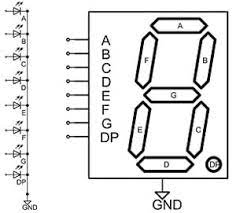
\includegraphics[width=0.75\textwidth]{figures/3.a.png}
    \caption
	{}
    \label{fig:fig1}
\end{figure}

 فرض می‌کنیم پایه‌های سون سگمنت نظیر به نظیر به درگاه \lr{A} متصل
شده‌اند. باتوجه به ساختار پایه‌ها در سون سگمنت، برای تولید کاراکترهای مذکور باید معادل باینری سگمنت‌هایی که قرار است روشن
شوند را محاسبه کنیم. پس به ترتیب داریم:
\lr{\lstinputlisting[language=C, showstringspaces=false, basicstyle=\ttfamily]{sources/3.c}}


\section*{منابع}
\renewcommand{\section}[2]{}%
\begin{thebibliography}{99} % assumes less than 100 references
%چنانچه مرجع فارسی نیز داشته باشید باید دستور فوق را فعال کنید و مراجع فارسی خود را بعد از این دستور وارد کنید


\begin{LTRitems}

\resetlatinfont

\bibitem{b1}

\end{LTRitems}

\end{thebibliography}


\end{document}
